\documentclass[a4paper]{article}

\usepackage[cm]{fullpage} % Package to use full page
\usepackage{parskip} % Package to tweak paragraph skipping
\usepackage{tikz} % Package for drawing
\usepackage{amsmath}
\usepackage{graphicx}
\usepackage{url}
\usepackage{verbatim}
\usepackage{subcaption}

\title{The Maths of Snakes and Ladders}
\author{J Campbell}
\date{\today}

\begin{document}

\maketitle
\section{Introduction}
Snakes and Ladders is an ancient Indian board game regarded today as a worldwide classic. It is played between two or more players on a gameboard having numbered, gridded squares. A number of 'ladders' and 'snakes' are pictured on the board, each connecting two specific board squares. The object of the game is to navigate one's game piece, according to die rolls, from the start (off the board) to the finish (square 100), helped or hindered by ladders and snakes respectively.\cite{wiki:ButterflyEffect}

\begin{figure}[!htbp]
\begin{center}
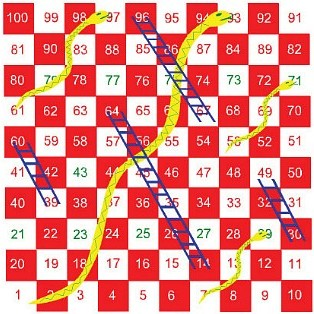
\includegraphics[scale=2.5]{images/SALboard}
\end{center}
\caption{The board that we will be studying.}
\label{board}
\end{figure}

\section{Markov Chains}
A Markov chain is a mathematical system that undergoes changes from one state to another. It is a random process in which the next state depends only on the current state and not on the sequence of events that preceded it. This is called the Markov property. This applies to Snakes and Ladders where a state is the position of a player on the board. To get to the next state you need to roll the die again and this is called a Transition. A Transition Matrix describes the probability distribution of all transitions.

Snakes and Ladders is actually an example of an Absorbing Markov Chain. This is because it has an absorbing state, a state which once entered, cannot be left. In this case it is when a player reaches $100$, the game ends.

\section{The Transition Matrix}
In this Transition Matrixix, the value of $M_{x,y}$ is the probability of moving from $x$ to $y$. Below is the code used in sage to create the matrix for Figure \ref{board}.

\begin{verbatim}
a = matrix(QQ, 101) # creates a square matrix populated with 0's
SaLdic = {29: 7, # a dictionary of all the snakes and ladders
          71: 53,
          93: 1,
          97: 61,
          14: 64,
          30: 49,
          39: 60,
          67: 96,
          }

def rolldie(N):
    """
    Simulates the rolling of a die
    Inputs: an integer N, the index of the row in the matrix
    Outputs: alters the matrix a to reflect the outcome of the die
    """
    for i in range(1,7):
        if N + i <= 100: # player must land on '100' exactly
            a[N, N + i] = 1/6
        else: # otherwise, player does not move
            a[N, N] += 1/6

for k in range(100): # does rolldie over the entire matrix except for [100,100].
    if k not in SaLdic: # except for snakes and ladders
        rolldie(k)

for p, q in SaLdic.iteritems(): # changes probabilities of moving along snake/ladder
    a[p, q] = 1                 # to 1 because they are certain.
\end{verbatim}

Then we can create a vector to represent the initial state. It begins with just $1$ in $Row_0$ because the probability of being off the board at the start of the game is certain. By multiplying this vector by the transition matrix, it gets populated by more and more probabilities.

\section{Limitations}
There is one big assumption made in this model though. It assumes that moving up/down a ladder/snake counts as a roll of the die instead of being instantaneous. This is not how the game is normally played but the overall effect is small.

However, this does make a large difference in computational speed. Matrix multiplication requires $n^3$ calculations and this particular board has a total of 8 ladders and snakes. If their corresponding rows and columns were removed from the transition matrix it would reduce the number of calculations required by $21.9\%$.
\begin{verbatim}
x = 101^3
y = (101-8)^3
(x - y)/float(x)*100
21.92990203833637
\end{verbatim}

\begin{figure}[!htbp]
\centering
\begin{subfigure}{.5\textwidth}
  \centering
  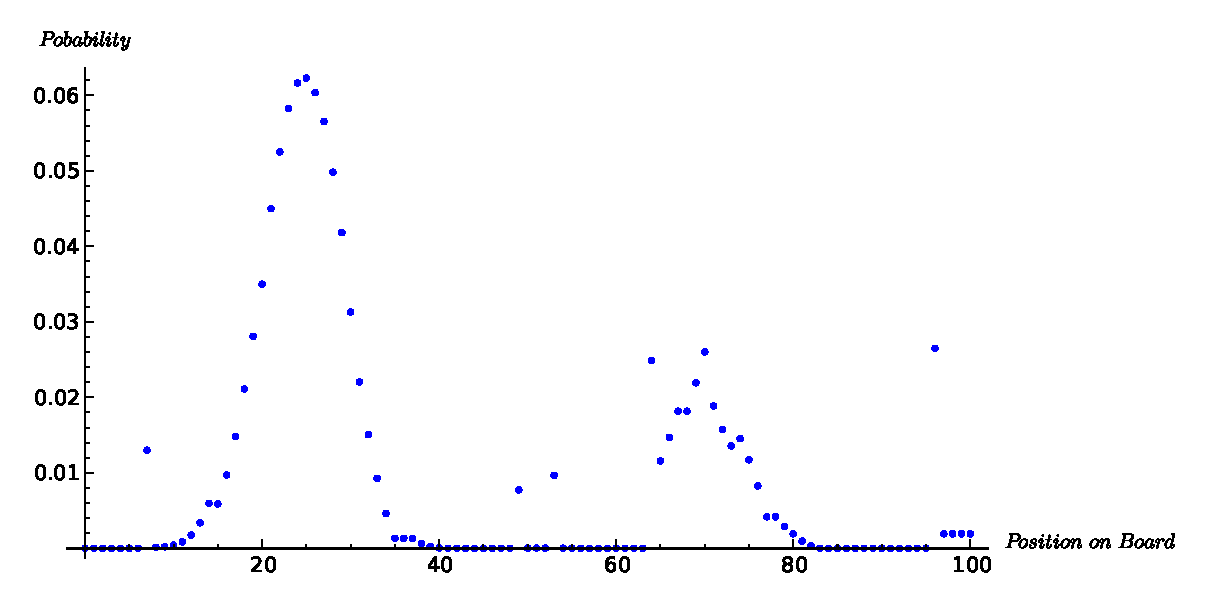
\includegraphics[width=\linewidth]{images/7plot}
  \caption{7 rolls}
  \label{7rolls}
\end{subfigure}%
\begin{subfigure}{.5\textwidth}
  \centering
  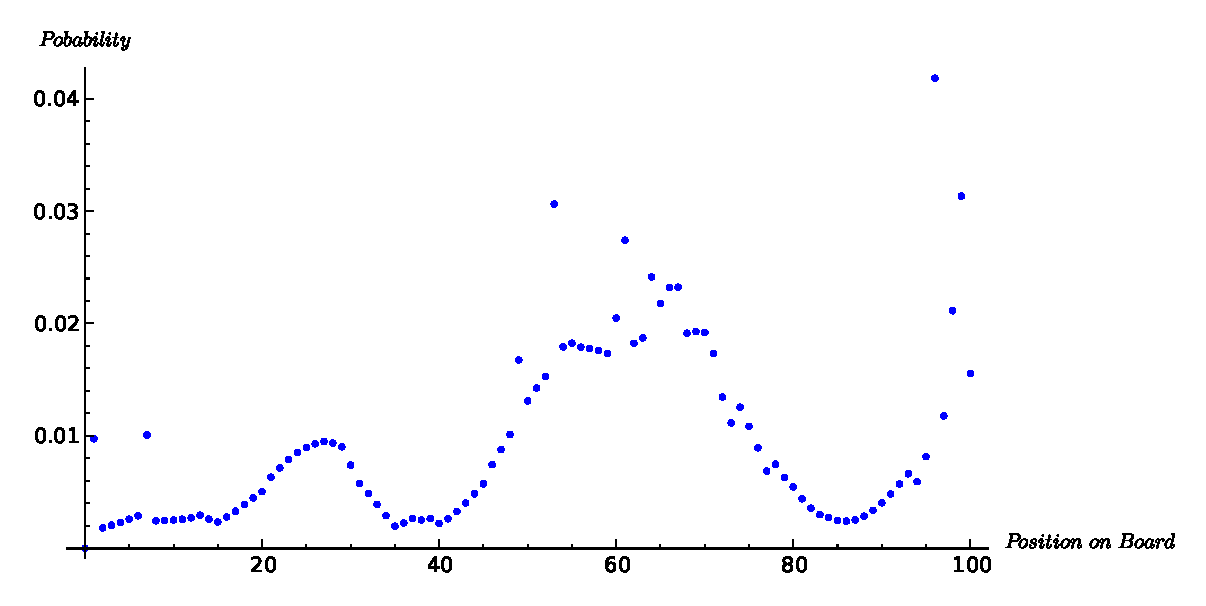
\includegraphics[width=\linewidth]{images/15plot}
  \caption{15 rolls.}
  \label{15rolls}
\end{subfigure}
\caption{The Probability Distributions after different numbers of rolls.}
\label{plots}
\end{figure}

\section{The Results}
In Figure \ref{plots} we can see the effect the snakes and ladders have on the probability distributions. We end up with several peaks in our graph due to players skipping large areas of the board with a ladder and then repeating areas due to a snake. Figure \ref{7rolls} shows us the first time a player might reach square 100. This is after only 7 rolls of the die. Figure \ref{15rolls} shows the probability distribution 8 rolls later and as you would expect it has a much more even spread. An interesting point is that square 1 has a relatively large probability, this is due to the long snake running across the board.

\begin{figure}[!htbp]
\centering
\begin{subfigure}{.5\textwidth}
  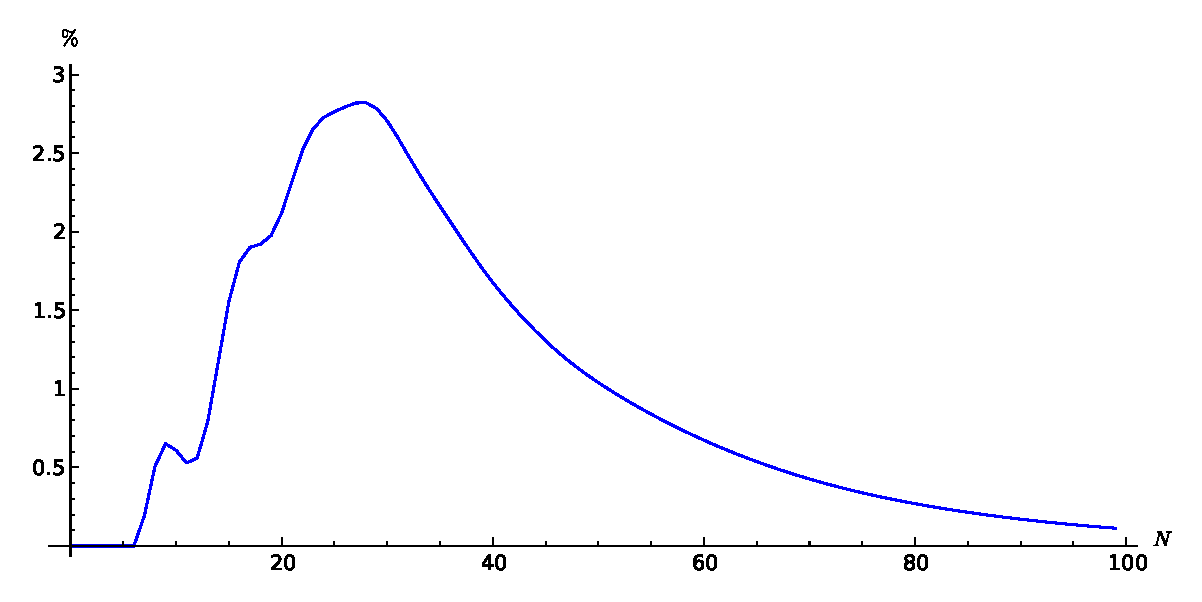
\includegraphics[width=\linewidth]{images/turns}
  \caption{The Percentage of games that end on turn $N$.}
  \label{rolls}
\end{subfigure}%
\begin{subfigure}{.5\textwidth}
  \centering
  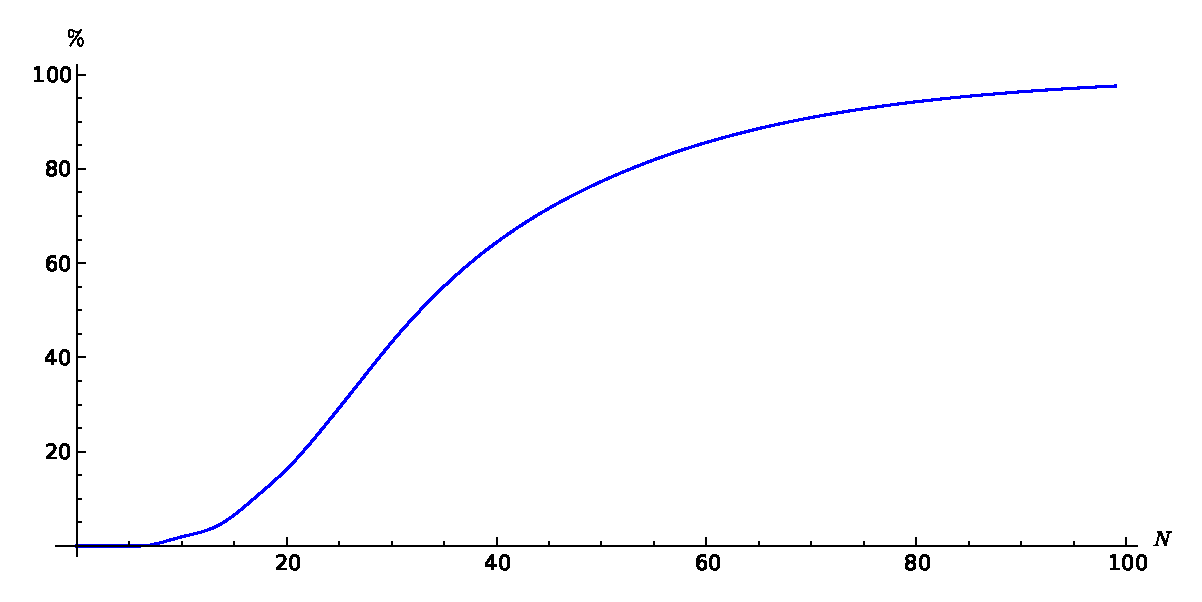
\includegraphics[width=\linewidth]{images/sumturns}
  \caption{The Percentage of games that end by turn $N$.}
  \label{sumrolls}
\end{subfigure}
\caption{Behaviour compared to $N$ rolls.}
\label{Nrolls}
\end{figure}

Figure \ref{Nrolls} is produced by repeatedly mutlipying by the Transition Matrix (rolling the die), taking the value at $Row_{100}$ and then appending it to a list.  Figure \ref{rolls} shows us that the modal value of $N$ is 28, ie. more games will be completed in 28 rolls than any other number of rolls. Figure \ref{sumrolls} is the same process done cumulatively. It tells us that the median is 33, ie. half of all games are completed in less than 33 rolls and half of all games are completed in 33 or more rolls.

\section{The Future}

If this project were to continue there are several new things could be done:
\begin{itemize}
    \item Improve the Transition Matrix so that it gave a more accurate representation of the game and therefore reduced calculation times.
    \item Create a function that generated different game boards with randomly placed snakes and ladders.
    \item Using a large set of random boards, look for patterns between game length and number of snakes/ladders. Also look at the properties of a more/less frequently used snake/ladder.
    \item Using the points previously mentioned, create a function that when given specific parameters (size of board, game length, number of snakes/ladders,...) will produce a random board with those properties.
\end{itemize}

\bibliographystyle{plain}
\bibliography{SALbib}
\end{document}